\chapter{Características numéricas de una distribución}

\section{Medidas de posición}

\begin{defi}[Esperanza]
Sea X una variable aleatoria y $F_X$ su función de distribución. Se define la esperanza de la distribución como
\begin{align*}
    E[X] = \int_{\mathbb{R}}{x \ dF_X(x)}.
\end{align*}
\end{defi}

\begin{prop}
Algunas propiedades de la esperanza.
\begin{enumerate}
    \item[(1)] Si X es una variable aleatoria tal que $P(X \ge 0) = 1$, entonces $E[X] \ge 0$.
    \item[(2)] Si X es una variable aleatoria tal que $P(X = c) = 1$, entonces $E[X] = c$.
    \item[(3)] Si X es una variable aleatoria tal que $P(a < X < b) = 1$, entonces $a < E[X] < b$.
    \item[(4)] Sea X una variable aleatoria y sea Y = a + bX, $a, b \in \mathbb{R}$. Si $E[X] < +\infty$, entonces $E[Y] = E[a] + E[bX] = a + bE[X] < +\infty$.
    \item[(5)] Sea X una variable aleatoria con función de distribución $F_X$ y sea Y = g(X) con g función medible. Entonces $E[Y] = \int_{\mathbb{R}}{g(x) \ dF_X(x)}$.
\end{enumerate}
\end{prop}

\begin{teo}[Teorema de König]
Sea X una variable aleatoria tal que $E[X^2] < +\infty$. El valor de $a \in \mathbb{R}$ que hace mínima $E[(X - a)^2]$ es $a = E[X]$.
\end{teo}

\begin{proof}
\begin{align*}
    E[(X - a)^2] &= E[(X - E[X] + E[X] - a)^2]\\
    &= E[(X - E[X])^2 + (E[X] - a)^2 + 2(X - E[X])(E[X] - a)] \\
    &= E[(X - E[X])^2] + E[(E[X] - a)^2] + 2E[(X - E[X])(E[X] - a)]
\end{align*}
Observamos que
\begin{enumerate}
    \item[(i)] $E[(X - E[X])^2] = V[X]$.
    \item[(ii)] $E[(E[X] - a)^2] = (E[X] - a)^2$, pues $(E[X] - a)^2$ es una constante.
    \item[(iii)] 
    \begin{align*}
        E[(X - E[X])(E[X] - a)] = (E[X] - a)E[X - E[X]] = (E[X] - a)(E[x] - E[x]) = 0.
    \end{align*}
\end{enumerate}
Por tanto
\begin{align*}
     E[(X - a)^2] = V[X] + (E[X] - a)^2.
\end{align*}
Nótese que $(E[X] - a)^2 \ge 0$, luego para que sea mínimo, $(E[X] - a)^2 = 0$, es decir, $a = E[X]$.
\end{proof}

\begin{defi}[Mediana]
Sea X una variable aleatoria con función de distribución $F_X$. M es una mediana de la distribución si verifica que
\begin{align*}
    P(X \leq M) \ge \frac{1}{2} \ \ \ y \ \ \ P(X \ge M) \ge \frac{1}{2}.
\end{align*}
Uniendo ambas condiciones, M es una mediana de la disitribución si
\begin{align*}
    \frac{1}{2} \leq F_X(M) \leq \frac{1}{2} + P(X = M).
\end{align*}
\end{defi}

\begin{defi}[Moda]
Sea X una variable aleatoria con función de distribució $F_X$. La moda, $M_0$, es el valor de mayor probabilidad (variable aleatoria discreta) o donde la función de densidad alcanza el maxímo (variable aleatoria absolutamente continua).
\end{defi}

\begin{defi}[Percentiles]
Sea X una variable aleatoria con función de distribució $F_X$. $P_{\alpha}$ es el percentil de orden $\alpha$ si
\begin{align*}
    P_X(X \leq P_{\alpha}) \ge \frac{\alpha}{100} \ \ \ y \ \ \ P_X(X \ge P_{\alpha}) \ge 1 - \frac{\alpha}{100}.
\end{align*}
\end{defi}

\begin{defi}[Cuartiles]
Son los percetiles de orden 25, 50 y 75, es decir, $Q_1 = P_{25}$, $Q_2 = P_{50}$ y $Q_3 = P_{75}$.
\end{defi}

\section{Medidas de dispersión}

\begin{defi}[Varianza]
Sea X una variable aleatoria con función de distribució $F_X$. Se define la varianza de la distribución como
\begin{align*}
    V[X] = E[(X - E[X])^2]
\end{align*}
siempre que $E[X^2] < +\infty$.
\end{defi}

\begin{obs} 
$V[X] = E[X^2] - (E[X])^2$.
\end{obs}

\begin{prop}
\begin{enumerate}
    \item[(i)] $V[X] \ge 0$ y $V[X] = 0$ si y solo si $P(X = a) = 1$.
    \item[(ii)] $V[a + bX] = b^2V[X]$.
\end{enumerate}
\end{prop}

\begin{proof}
Veamos $(ii)$. 
\begin{align*}
    V[a + bX] &= E[(a + bX - E[a + bX])^2] = E[(a + bX - a + bE[X])^2] \\
    &= E[b^2(X - E[X])^2] = b^2E[(X - E[X])^2]\\
    &= b^2V[X].
\end{align*}
\end{proof}

\begin{defi}[Desviación típica]
Sea X una variable aleatoria. Se define la desviación típica como $D(X) = +\sqrt{V(X)}$.
\end{defi}

\begin{obs}
Si X es una variable aleatoria con $V[X]$ conocida, entonces
\begin{align*}
    Y = \frac{X - E[X]}{D(X)}
\end{align*}
es una variable aleatoria con $E[Y] = 0$ y $V[Y] = 1$.
\end{obs}

\begin{teo}[Desigualdad de Chebyshev]
Sea X una variable aleatoria con $E[X]$ y $V[X]$ conocidas. Entonces
\begin{align*}
    P(|X - E[X]| \leq aD(x)) \ge 1 - \frac{1}{a^2}
\end{align*}
para todo $a > 0$.
\end{teo}

\section{Medidas de asimetría}

\begin{defi}
Una variable aleatoria X tiene un disrtibución simétrica respecto del origen si $X$ y $-X$ tienen la misma función de distribución (es decir, otorgan misma probabilidad a mismos conjuntos).
\end{defi}

\begin{defi}
Una variable aleatoria X tiene una distribución simétrica respecto $a \in \mathbb{R}$ si $X - a$ y $a - X$ tienen la misma función de distribución.
\end{defi}

\begin{obs}
Sea X variable aleatoria y sea $E[X]$. Entonces
\begin{enumerate}
    \item[(i)] $M_1 = E[X - E[X]] = E[x] - E[X] = 0$.
    \item[(ii)] $M_2 = E[(X - E[X])^2]$.
    \item[(iii)] $M_3 = E[(X - E[X])^3]$. Si X es simétrica respecto $\mu = E[X]$, entonces $M_3 = 0$, es más, $M_r = 0$ para $r$ impar.
\end{enumerate}
\end{obs}

\begin{defi}[Coeficiente de asimetría]
\begin{align*}
    CA = \frac{M_3}{(D(X))^2},
\end{align*}
\begin{enumerate}
    \item[(i)] Si $CA = 0$, entonces X es simértica.
    \item[(ii)] Si $CA < 0$, entonces X es asimétrica a la izquierda.
    \item[(iii)] Si $CA > 0$, entonces X es asimétrica a la derecha.
\end{enumerate}
\end{defi}

\begin{align*}
    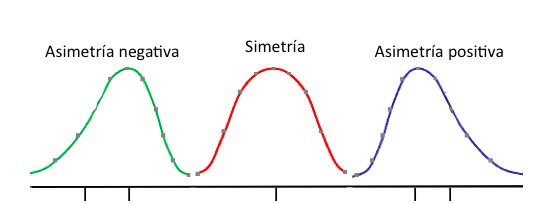
\includegraphics[width=0.7\textwidth]{coeficiente de asimetria.jpg}
\end{align*}

\section{Coeficientes de apuntalamiento}

\begin{defi}[Coeficiente de apuntalamiento]
\begin{align*}
    CA_p = \frac{M_4}{(D(x))^4} - 3.
\end{align*}
\end{defi}

\begin{obs}
\begin{enumerate}
    \item[(i)] $M_4 = E[(X - E[X])^4]$.
    \item[(ii)] Si $X \sim N(0,1)$ entonces $CA_p = 0$.
\end{enumerate}
\end{obs}